\documentclass[aspectratio=169]{beamer}
\usepackage[utf8]{inputenc}
\usepackage{amsmath}
\usepackage{tikz}
\usepackage{opensans}

\title{Differentiability}
\author{Paulo Fagandini}
\institute{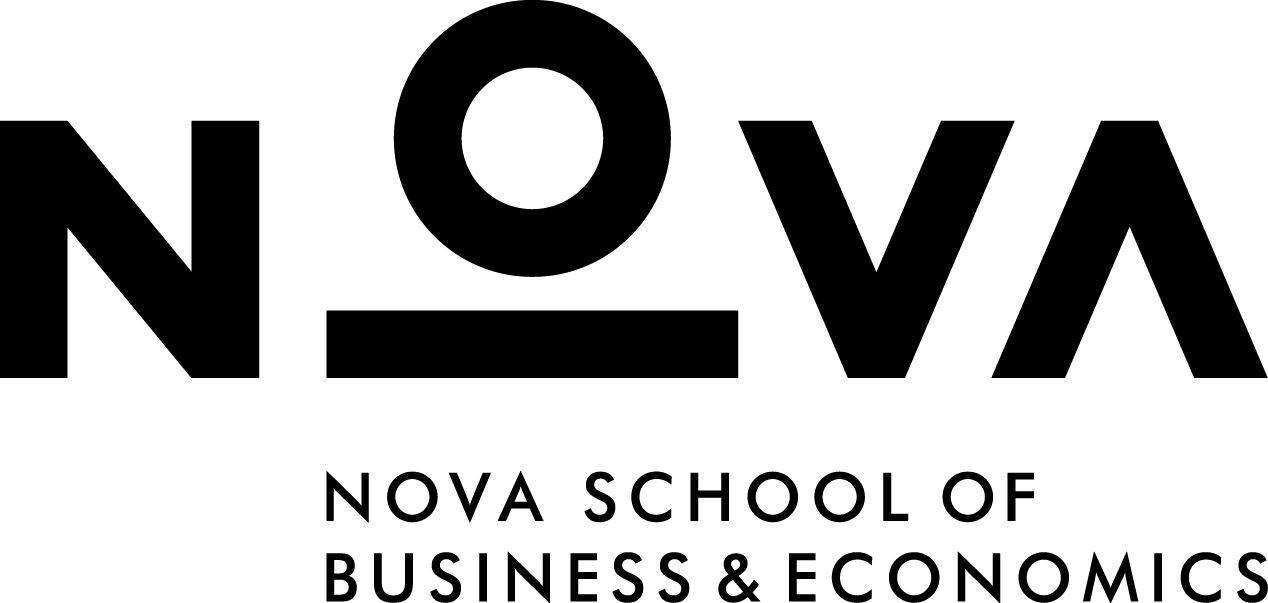
\includegraphics[scale=0.3]{NovaPrincipalV1.png}}
\date{}

\makeatletter
\setbeamertemplate{theorem begin}{%
  \setbeamercolor{block title}{bg=white,fg=black}%
  \setbeamercolor{itemize item}{fg=black}%
  \setbeamercolor{itemize subitem}{fg=black}%
  \setbeamercolor{itemize subsubitem}{fg=black}%
  \setbeamercolor{enumerate item}{fg=black}%
  \setbeamercolor{enumerate subitem}{fg=black}%
  \setbeamercolor{enumerate subsubitem}{fg=black}%
  \begin{\inserttheoremblockenv}
    {%
      \textbf{\inserttheoremname}
      %\inserttheoremnumber
      \ifx\inserttheoremaddition\@empty\else\ \inserttheoremaddition\fi%
    }%
    \normalfont%
}

\setbeamertemplate{theorem end}{%
    \end{\inserttheoremblockenv}%
}

\setbeamercolor{block title}{bg=white,fg=black}%
\setbeamercolor{itemize item}{fg=black}%
\setbeamercolor{itemize subitem}{fg=black}%
\setbeamercolor{itemize subsubitem}{fg=black}%
\setbeamercolor{enumerate item}{fg=black}%
\setbeamercolor{enumerate subitem}{fg=black}%
\setbeamercolor{enumerate subsubitem}{fg=black}%

\makeatother

\newtheorem{defenition}{Definition}[section]
\newtheorem{proposition}{Conjecture}[section]

\AtBeginSection{\frame{\sectionpage}}

\setbeamertemplate{footline}{
    \hspace{0.05\textwidth}
    \raisebox{3ex}{\insertshortauthor{}}\hfill
    \raisebox{3ex}{\insertframenumber{}/\inserttotalframenumber} \hfill
    {\raisebox{3ex}{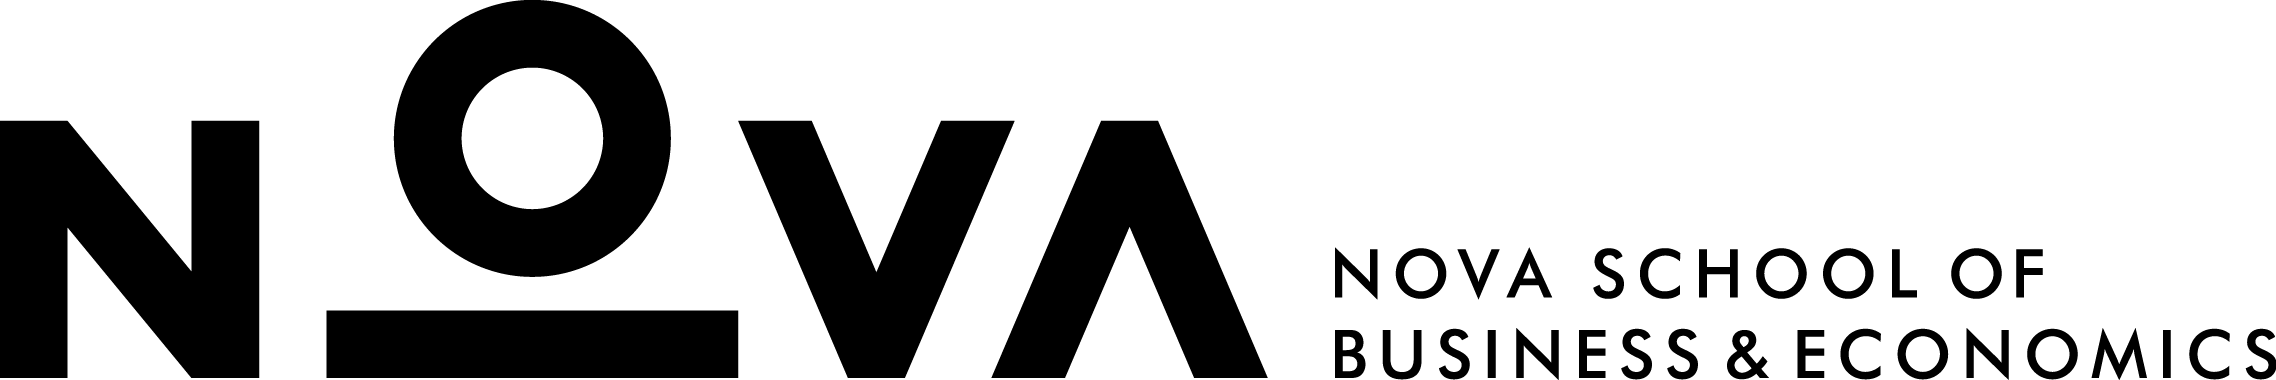
\includegraphics[height=0.04\textheight]{NovaPrincipalV2.png}}}
    \hspace{0.05\textwidth}
}

\setbeamertemplate{navigation symbols}{}

\setbeamercolor{title}{fg = black}
\setbeamercolor{subtitle}{fg = black}
\setbeamercolor{frametitle}{fg = white, bg = black}

\hypersetup{linkcolor=black, colorlinks=true}

\begin{document}

{
\setbeamertemplate{footline}{} 
\begin{frame}
  \titlepage
\end{frame}
}

\begin{frame}
   \begin{definition}
        The function $f:\mathbb{R}\rightarrow\mathbb{R}$ is \textbf{differentiable} in $\hat{x}\in\mathbb{R}$ if the limit
        \begin{align*}
            \lim_{h\rightarrow 0}\frac{f(\hat{x}+h)-f(\hat{x})}{h}
        \end{align*}
        exists. If it does, we denote it as $\frac{df(\hat{x})}{dx} $, or $f'(\hat{x})$, or $f_x(\hat{x})$.
   \end{definition}
\end{frame}

\begin{frame}
    \begin{definition}
        The function $f:\mathbb{R}^n\rightarrow \mathbb{R}$ is \textbf{partially differentiable} in $\hat{x}=(\hat{x}_1,\hat{x}_2,\ldots,\hat{x}_n)$ with respect to $x_j$ if the limit
        
        \begin{align*}
            \lim_{h\rightarrow 0}\frac{f(\hat{x}_1,\ldots,\hat{x}_j+h,\hat{x}_{j+1},\ldots,\hat{x}_n)-f(\hat{x}_1,\ldots,\hat{x}_{j},\hat{x}_{j+1},\ldots,\hat{x}_n)}{h}
        \end{align*}
        exists. If it does, we denote it as $\frac{\partial f(\hat{x})}{\partial x_j} $, or $f_{x_j}(\hat{x})$.
    \end{definition}
\end{frame}

\begin{frame}
\begin{definition}
    If $f:\mathbb{R}^n\rightarrow\mathbb{R}$ is partially differentiable in each coordinate of $\hat{x}$, then its \textbf{gradient} is defined as:
    
    \begin{align*}
        \nabla f(\hat{x}) = \left(\begin{array}{c}\frac{\partial f(\hat{x})}{\partial x_1}\\ \vdots \\ \frac{\partial f(\hat{x})}{\partial x_i} \\ \vdots \\ \frac{\partial f(\hat{x})}{\partial x_n}\end{array}\right)
    \end{align*}
\end{definition}
\end{frame}

\begin{frame}
    \begin{definition}
        If $f:\mathbb{R}^n\rightarrow\mathbb{R}^m$ is partially differentiable in each coordinate of $\hat{x}$, then the \textbf{Jacobian} matrix (also denoted $\nabla f$, and $D f$) is defined as:
    
    \begin{align*}
        \nabla f(\hat{x}) = \left(\begin{array}{cccc}\frac{\partial f_1(\hat{x})}{\partial x_1} & \frac{\partial f_1(\hat{x})}{\partial x_2} & \ldots & \frac{\partial f_1(\hat{x})}{\partial x_n} \\
        \frac{\partial f_2(\hat{x})}{\partial x_1} & \frac{\partial f_2(\hat{x})}{\partial x_2} & \ldots & \frac{\partial f_2(\hat{x})}{\partial x_n} \\
        \vdots & \vdots & \ddots & \vdots \\
        \frac{\partial f_m(\hat{x})}{\partial x_1} & \frac{\partial f_m(\hat{x})}{\partial x_2}& \ldots & \frac{\partial f_m(\hat{x})}{\partial x_n}
        \end{array}\right)
    \end{align*}
    where in this case $f_i(\hat{x})$ represents the coordinate $i$ of $f(\hat{x})$.
    \end{definition}
\end{frame}

\begin{frame}
    \begin{definition}
    
    The \textbf{higher order derivative} is defined recursively, consider the derivative of $f$, of order $n$, on $\hat{x}$ as,
    \begin{align*}
      f^{(n)}(\hat{x})&=(f^{(n-1)}(\hat{x}))'\\
      f^{(1)}(\hat{x})&=f'(\hat{x})  
    \end{align*}
    
    \end{definition}
    
    \begin{definition}
        The second partial derivative is defined as:
        
        \begin{align*}
            \frac{\partial^2f(\hat{x})}{\partial x_i \partial x_j}  := \frac{\partial}{\partial x_i}\left(\frac{\partial f(\hat{x})}{\partial x_j}\right)
        \end{align*}
        It is well defined if both limits exist.
    \end{definition}
\end{frame}

\begin{frame}
    \begin{definition}
        The \textbf{Hessian} of a function $f$ is the matrix with the second partial derivatives of $f$.
        
        \begin{align*}
            H(f,\hat{x})=\left(
            \begin{array}{cccc}
                \frac{\partial^2f(\hat{x})}{(\partial x_1)^2} & \frac{\partial^2f(\hat{x})}{\partial x_2\partial x_1}&\ldots&\frac{\partial^2f(\hat{x})}{\partial x_n\partial x_1}\\
                \frac{\partial^2f(\hat{x})}{\partial x_2\partial x_1} & \frac{\partial^2f(\hat{x})}{(\partial x_2)^2} & \ldots & \frac{\partial^2f(\hat{x})}{\partial x_2\partial x_n}\\
                \vdots & \vdots &\ddots & \vdots\\
                \frac{\partial^2f(\hat{x})}{\partial x_n\partial x_1} & \frac{\partial^2f(\hat{x})}{\partial x_n\partial x_2}&\ldots &\frac{\partial^2f(\hat{x})}{(\partial x_n)^2}
            \end{array}
            \right)
        \end{align*}
        
    \end{definition}
\end{frame}

\begin{frame}

\begin{proposition}
    Let $f,g:\mathbb{R}\rightarrow\mathbb{R}$ differentiable, it holds that:
    
    \begin{enumerate}
        \item $(f+g)'(x)=f'(x)+g'(x)$
        \item $(f\cdot g)'(x)=f'(x)g(x)+f(x)g'(x)$
        \item $\left(\frac{f}{g}\right)'(x)=\frac{f'(x)g(x)-f(x)g'(x)}{g(x)^2}$
        \item If $h(x)=f(g(x))$, then $h'(x)=f'(g(x))\cdot g'(x)$. The glorious \textbf{chain rule!}.
        \item Let $f:\mathbb{R}^n\rightarrow\mathbb{R}$ and $g:\mathbb{R}^k\rightarrow\mathbb{R}^n$. Now let $h:\mathbb{R}^k\rightarrow\mathbb{R}$ as $h(x)=f(g(x))$, with $x=(x_1,\ldots, x_j,\ldots, x_k)$.
        
        \begin{align*}
            \frac{\partial h}{\partial x_j} = \sum_{i=1}^n \frac{\partial f(x)}{\partial (g(x))_i}\frac{\partial (g(x))_i}{\partial x_j}
        \end{align*}
        
        With $(g(x))_i$ the coordinate $i$ of the vector $g(x)\in\mathbb{R}^n$.
    \end{enumerate}
\end{proposition}
    
\end{frame}

\begin{frame}
    
    \begin{theorem}[{Implicit Function}]
        Let $f:\mathbb{R}^n\rightarrow\mathbb{R}$ a function such that $f(z)=0$, with $z=(z_1,z_2,...,z_n)$. 
        
        If $f_{x_1}(z)\neq 0$, then there exists a differentiable function $g:\mathbb{R}^{n-1}\rightarrow\mathbb{R}$ such that $z_1=g(z_2,z_3,...,z_n)$, and $f(g(z_2,...,z_n),z_2,...,z_n)=0$ for any $(x_2,...,x_n)$ near $(z_2,...,z_n)$.
    \end{theorem}
    
\end{frame}

\begin{frame}
    
    \begin{theorem}[Intermediate Value]
        Consider a differentiable function $f:[a,b]\rightarrow\mathbb{R}$, then there is $c\in[a,b]$ such that $$f'(c)=\frac{f(b)-f(a)}{b-a}$$
    \end{theorem}
    
\end{frame}

\begin{frame}
    \begin{definition}
        $f:\mathbb{R}^n\rightarrow\mathbb{R}^n$ is called \textbf{locally Lipschitz continuous} if for any $x_0\in\mathbb{R}^n$, there is a neighborhood $V_{x_0}$ and a constant $L>0$ such that for any $x,y\in V_{x_0}$ it holds that $$||f(x)-f(y)||\leq L ||x-y||$$ $L$ is called the \textbf{Lipschitz constant}.
        
        If $L$ does not depend on $x_0$, it is called simply a \textbf{Lipschitz continuous}, and furthermore, if $L<1$ it is called a \textbf{contraction}.
    \end{definition}
\end{frame}

\begin{frame}
\begin{theorem}[Banach fixed point]
    If $f:\mathbb{R}^n\rightarrow\mathbb{R}^n$ is a contraction, then there is a single $x^*\in\mathbb{R}^n$ such that $f(x^*)=x^*$.
\end{theorem}
\end{frame}

\begin{frame}
    \begin{theorem}[Brower fixed point in $\mathbb{R}^n$]
        Consider $B_n\subseteq\mathbb{R}^n$ the unit open ball (an open ball of radius 1). Let $f:B_n\rightarrow B_n$ continuous. Then $f$ has a fixed point in $B_n$, that is, there is $x^*\in B_n$ such that $f(x^*)=x^*$.
    \end{theorem}
    
\end{frame}

\begin{frame}
    \begin{proposition}
        Let $f:\mathbb{R}\rightarrow\mathbb{R}$ be differentiable. $f$ is strictly increasing if and only if $f'(x)>0$ for any $ x\in\mathbb{R}$.
    \end{proposition}
\end{frame}

\begin{frame}

\begin{definition}
    Given $x_0\in\mathbb{R}$ and $f:\mathbb{R}\rightarrow\mathbb{R}$ differentiable (at least $k$ times). The $k-order$ Taylor series at $x_0$ is:
    
    \begin{align*}
        T(x_0,f)(x):=\sum_{i=0}^k \frac{f^{(i)}(x_0)}{i!}(x-x_0)^i
    \end{align*}
\end{definition}
    
\end{frame}

\begin{frame}

\begin{proposition}[l'H\^ opital's rule]

Let $f$ and $g$ be differentiable functions such that one of the following two conditions hold:

\begin{itemize}
    \item $\lim_{x\rightarrow x_0} f(x)=0$ and $\lim_{x\rightarrow x_0} g(x)=0$, or
    \item $\lim_{x\rightarrow x_0} |f(x)|=\infty$ and $\lim_{x\rightarrow x_0} |g(x)|=\infty$.
\end{itemize}
    
    Then $\lim_{x\rightarrow x_0} \frac{f(x)}{g(x)}=\lim_{x\rightarrow x_0} \frac{f'(x)}{g'(x)}$.
    
\end{proposition}
\end{frame}

\end{document}
